\documentclass[journal]{../IEEEtran}

\usepackage{graphicx}
\usepackage{fancyhdr}
\usepackage{epsfig} % for postscript graphics files
\usepackage{graphics} % for pdf, bitmapped graphics files

\graphicspath{{Figures/}}

\pagestyle{fancy}
\lhead{CPE 470/670}
\rhead{\thepage}
\chead{Team 6: Lab 6 Report}
\lfoot{}
\rfoot{}
\cfoot{}

\begin{document}

\begin{titlepage}
    \vspace*{\fill}
    \begin{center}
      {\LARGE \bf Lab 6: Ball Sorting Contest}

      {Team 6: Alexander  C. Woods and Taylor Mansfield}

      November 5, 2014
    \end{center}
    \vspace*{\fill}
  \end{titlepage}


\section{Hardware and Software Design}\label{S.design}
\IEEEPARstart{F}{inding}, capturing, and sorting balls in an arena in which the balls can potentially move is a very challenging problem. A robot must have an effective search pattern, reliably sense when a ball is within range of the grasping mechanism, be able to capture the ball and sense the color, and finally it must know where it is in order to properly sort the ball by dropping it over the appropriate side of the arena.

Mechanically, this problem present many challenges. Because two of the maximum of three motors are taken up by the drivetrain, only one motor remains to facilitate capturing, holding and dropping balls over the side. This limitation generally leads to a mechanism which can passively push the ball over the edge without any use of the motor, such as a ramp in the front of the robot. The ball is pushed over the edge by running the robot into the wall, forcing the ball up the ramp and eventually over the edge. This method has limitations in that if the robot is not perpendicular to the wall, the ball may not make it over the wall but rather will pop out the side of the ramp. Additionally, if the robot does not have enough speed when running into the wall, the ball may not have enough momentum to make it over.

For the capturing mechanism, a claw is positioned above the ramp which uses a motor to close on a ball when one is sensed. This claw also has a color sensor attached to it which can sense the presence of a ball when in the open position, and can sense the specific color of the ball when closed. This information is used by the robot in the sorting process to determine which side of the field to drop the ball over. All throughout the sorting process, the claw remains closed on the ball to keep it from rolling away from the robot. 

Even considering the limitations of the ramp and claw, this solution is the one of the best available and was utilized for the contest. As shown in Fig.~\ref{F.ramp}, the robot has a ramp at the front of the robot, and a claw above which descends on the ball to hold onto it during the sorting process. 

\begin{figure}[ht]
\centering
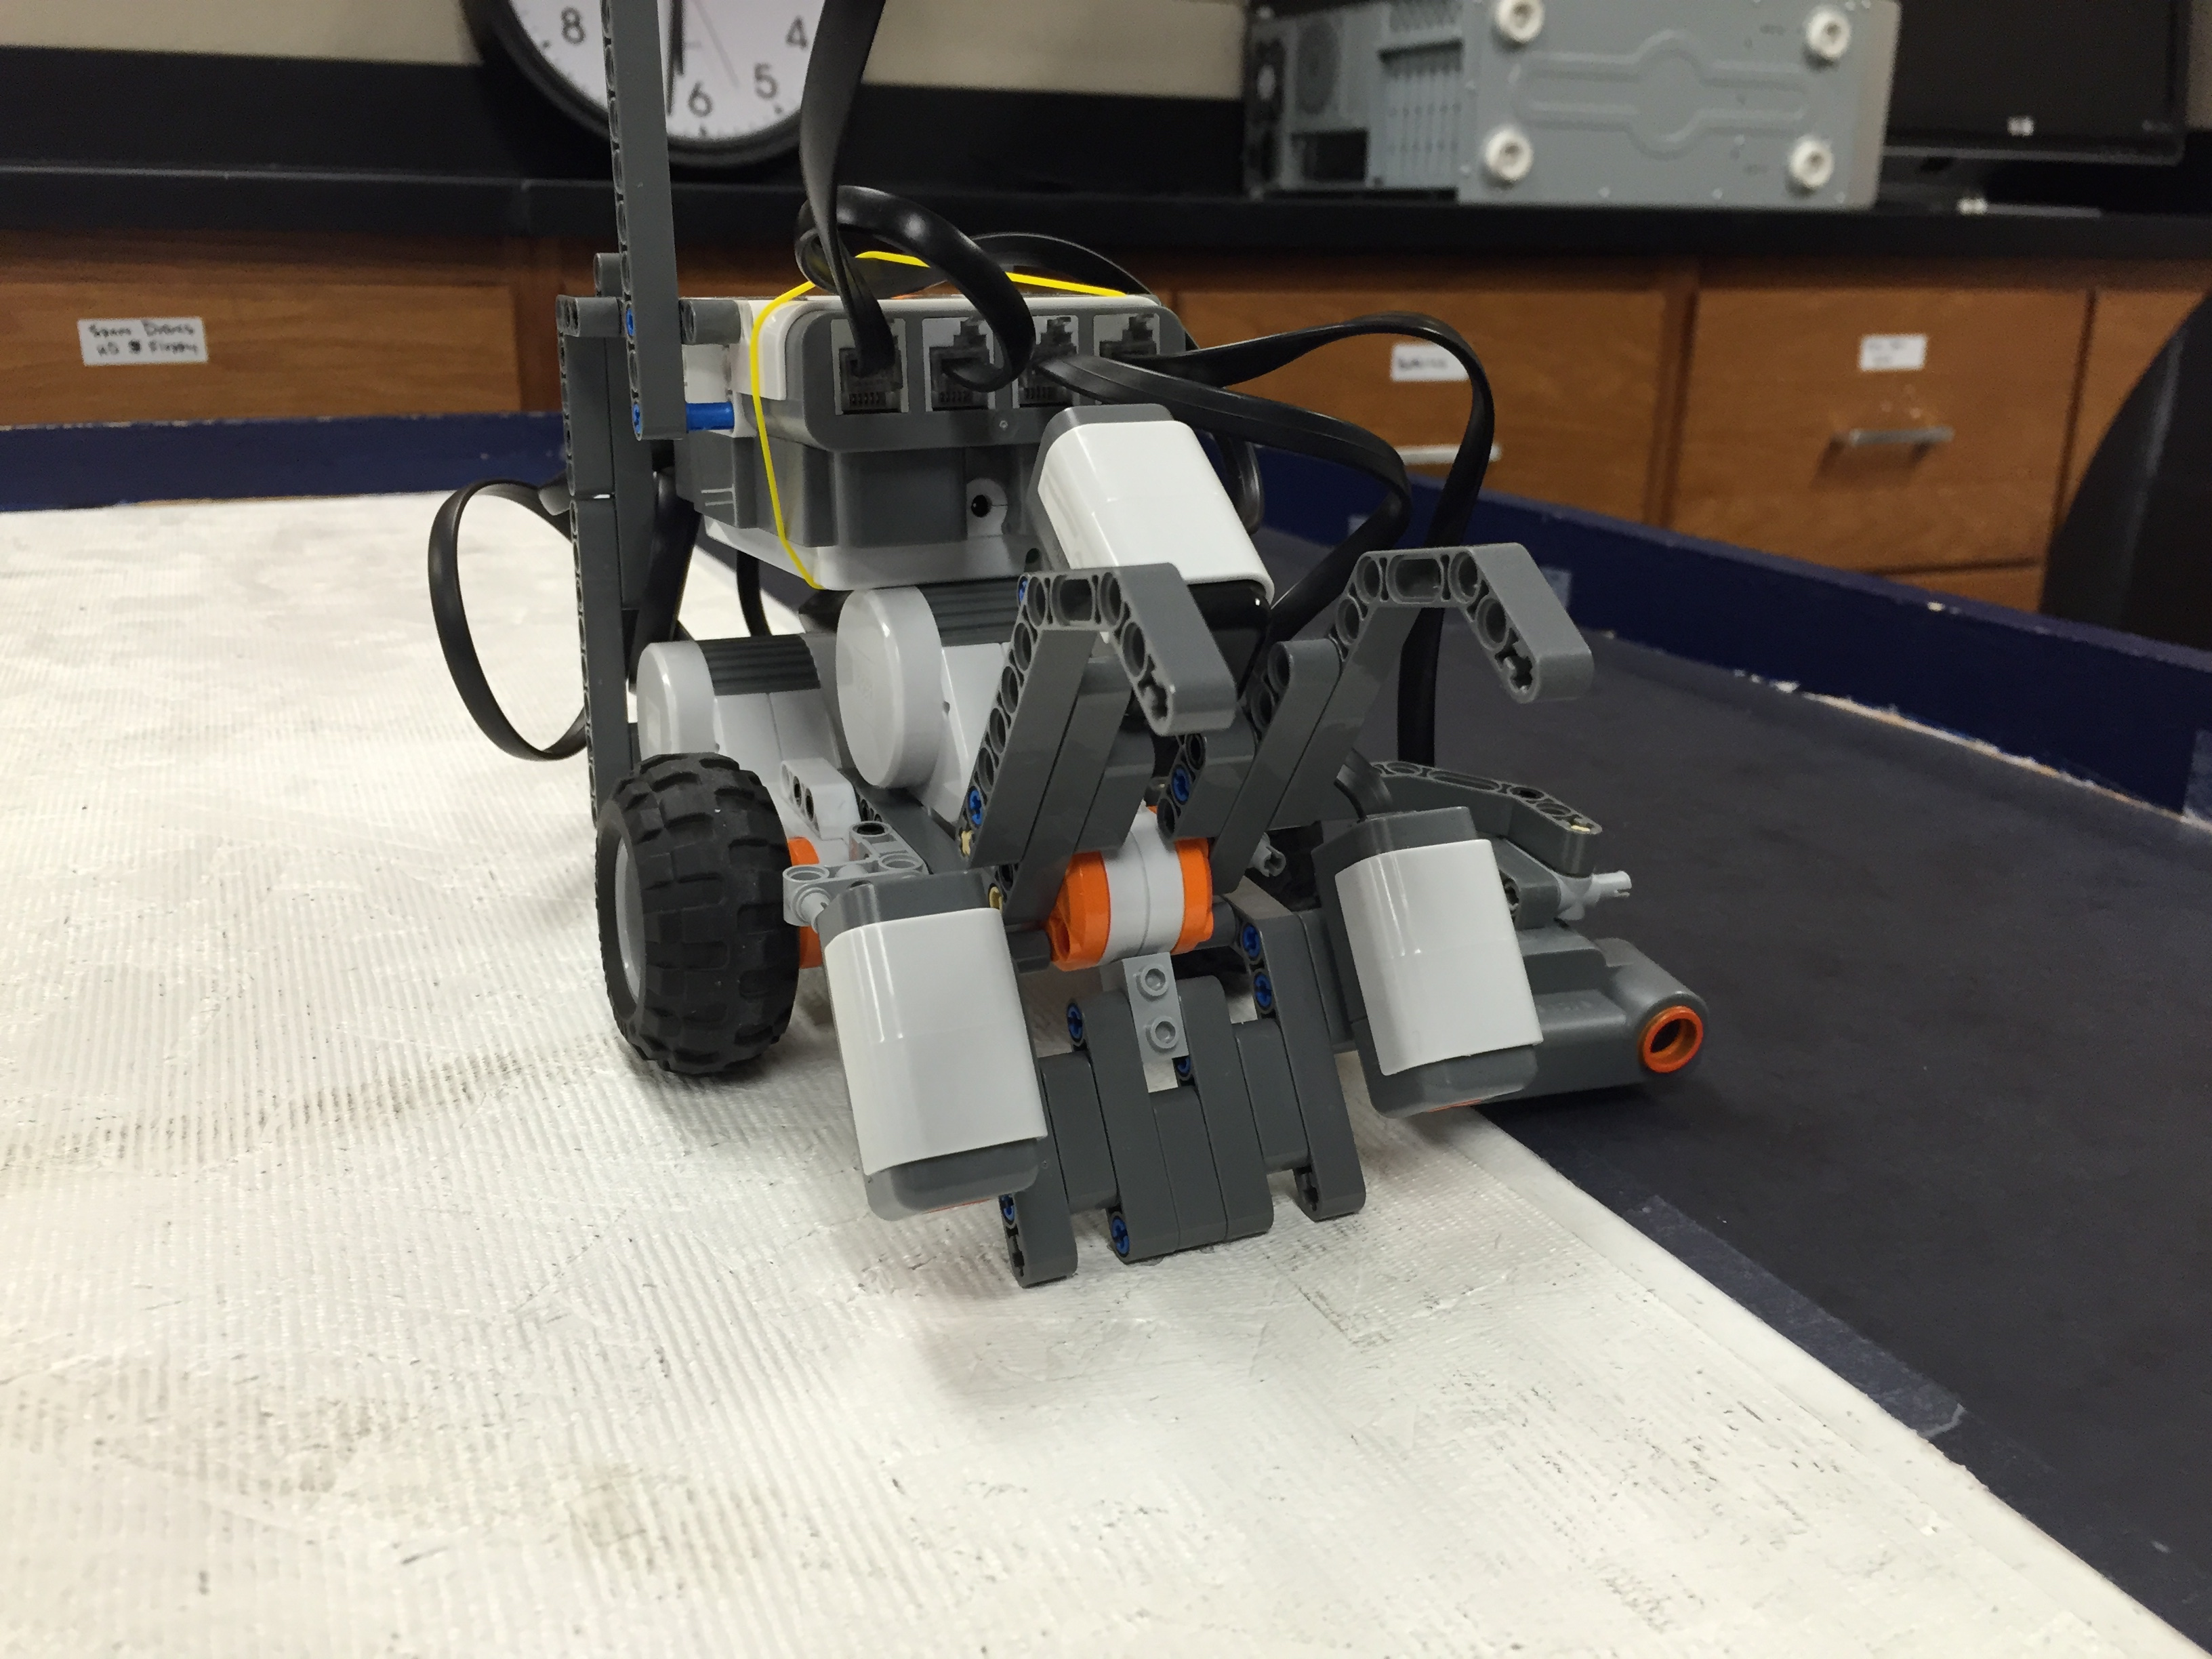
\includegraphics[width=1\columnwidth]{ramp.jpg}\\
\caption{The robot is equipped with a ramp which can push balls over the edge when rammed against a wall. Additionally, the robot has a claw which can descend on a ball to secure it during the sorting process.}
\label{F.ramp}
\end{figure}

The sensors used are kept to a minimum to keep the robot as simple as possible while maintaining full functionality. A compass sensor is used to provide the robot with heading information throughout the contest. The compass sensor is put through a quick calibration at the beginning of each contest to learn which headings aligned with the home and destination locations. The heading information is used throughout the contest to let the robot know which way it is facing.

An ultrasonic sensor is equipped which lets the robot sense and avoid wall while it is looking for balls. The ultrasonic sensor is strategically located on the left side of the robot as shown in Fig.~\ref{F.us_sensor} so that it can sense walls, but will not be fooled by a ball. This is because the robot keeps the wall on its left side naturally. If the robot were to use a right sided wall following technique instead the ultrasonic sensor would be located on the other side of the robot.

\begin{figure}[ht]
\centering
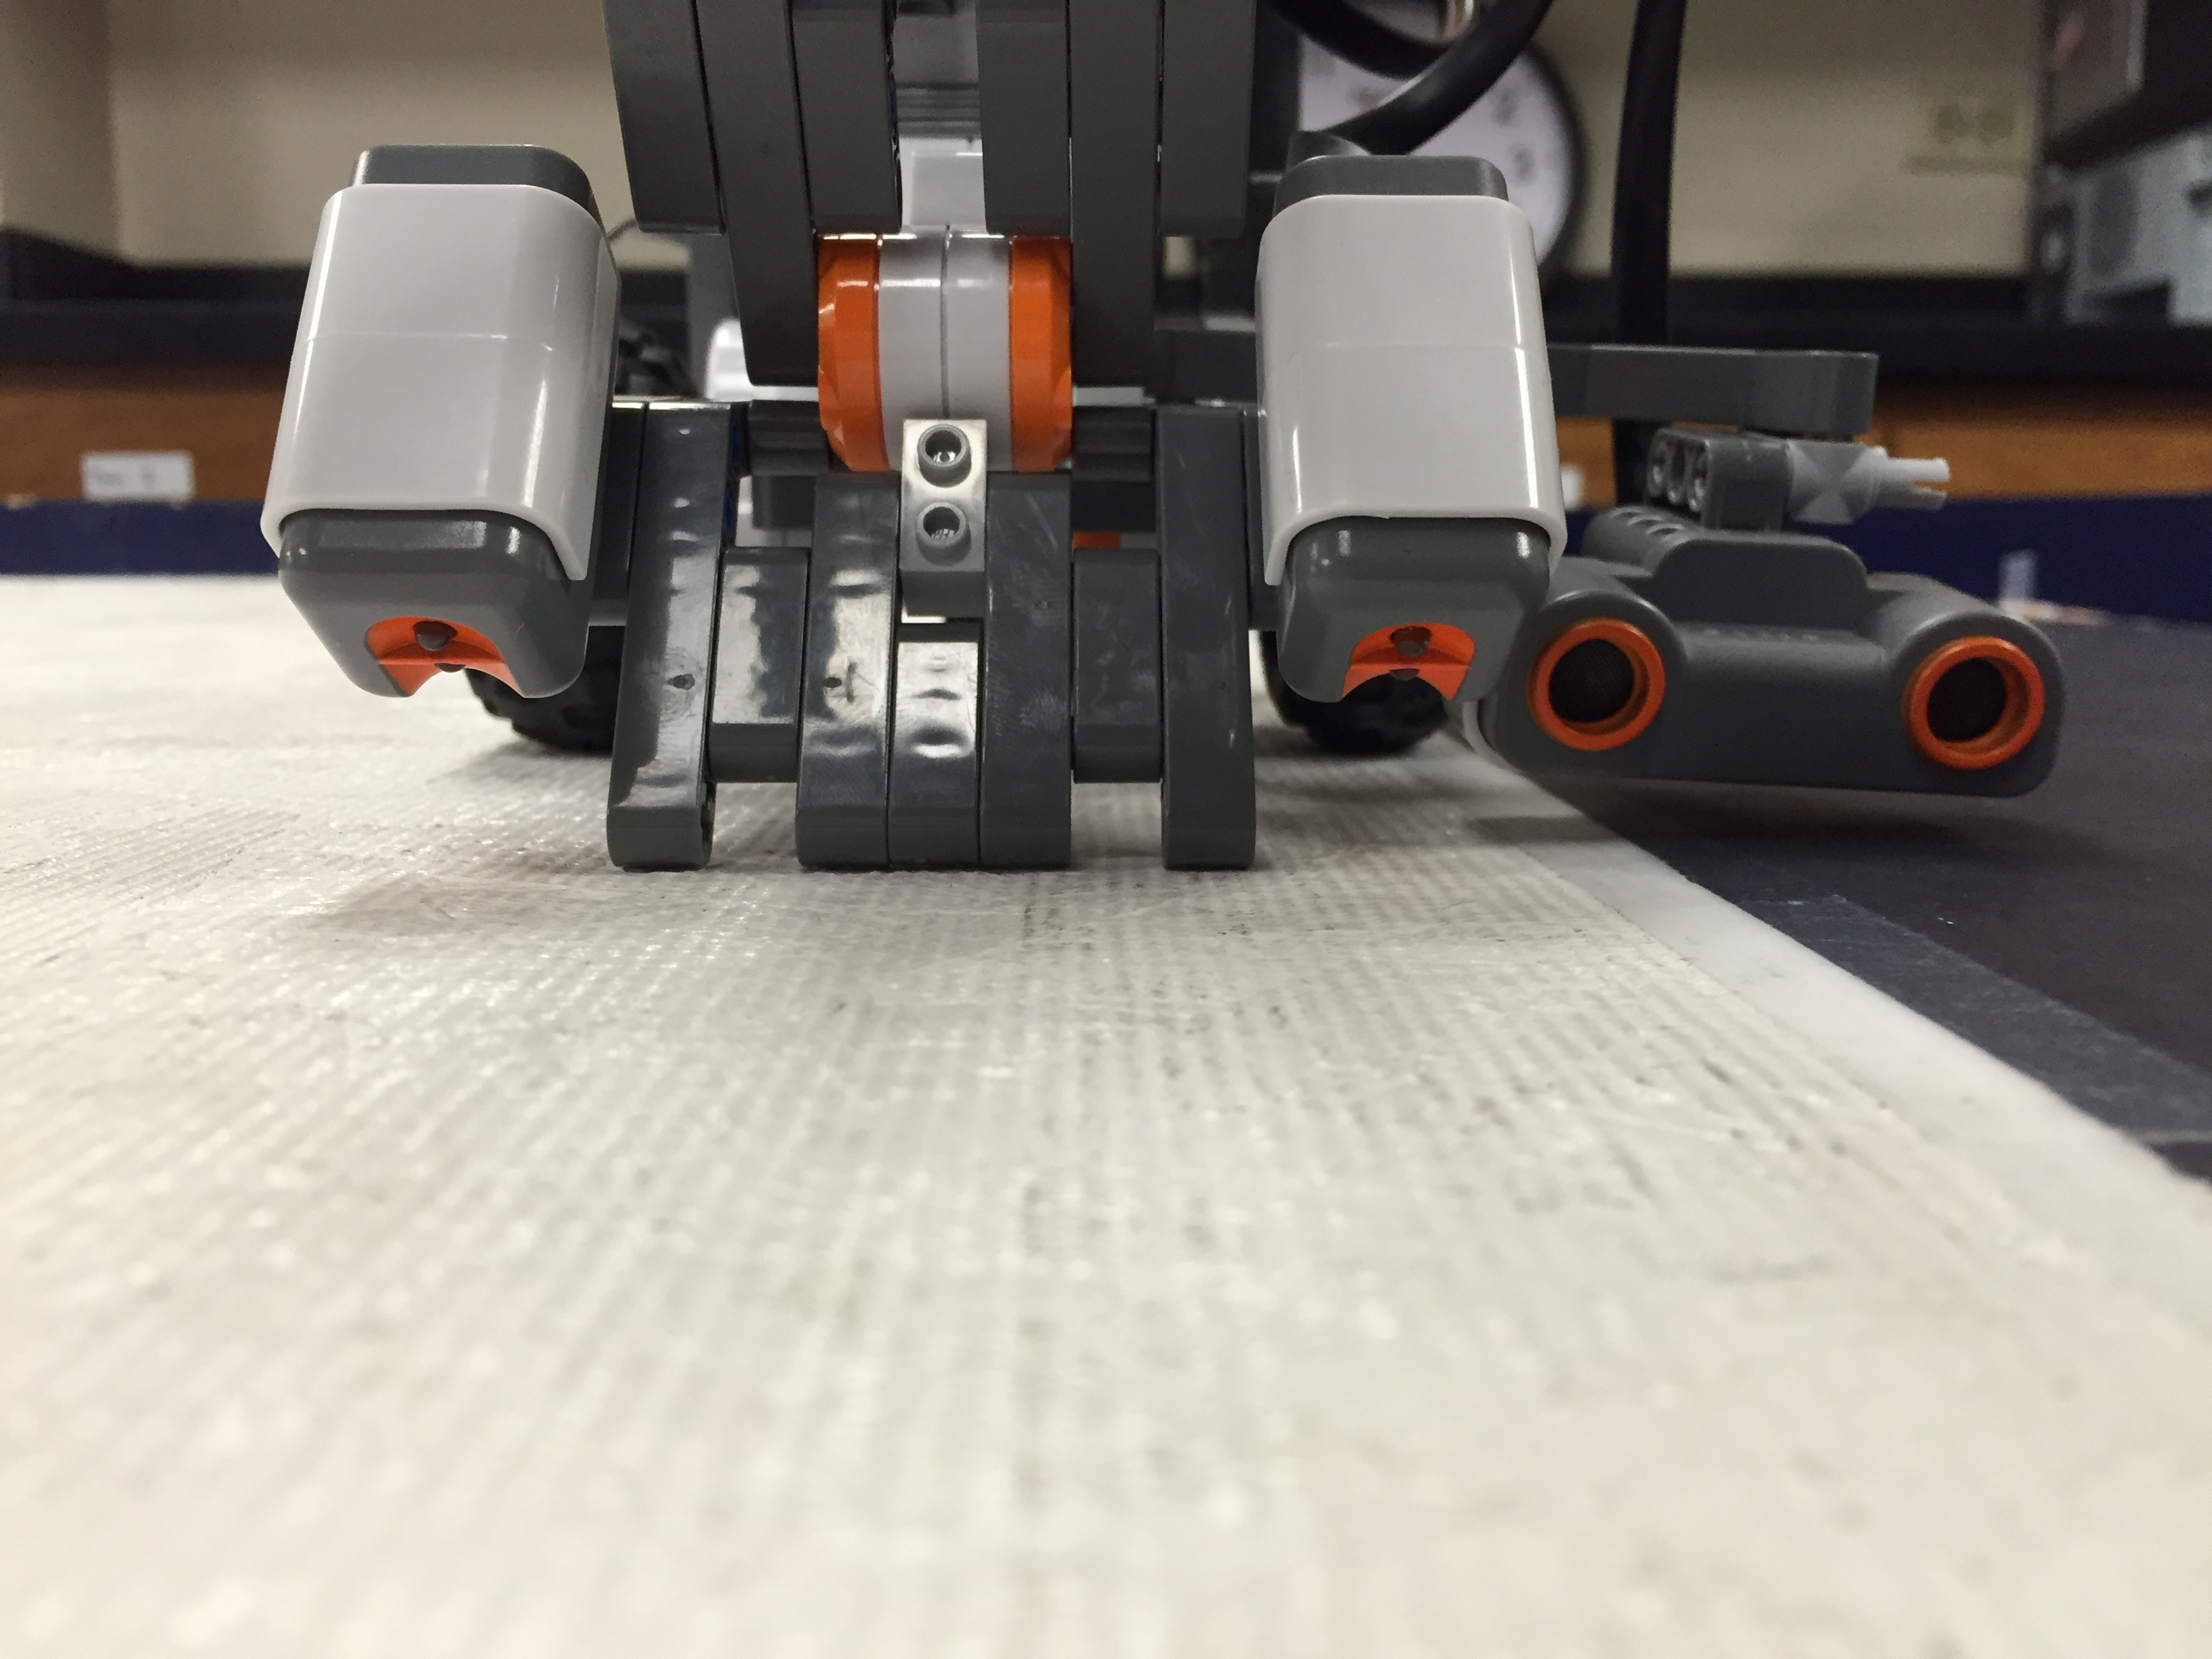
\includegraphics[width=1\columnwidth]{us_sensor.jpg}\\
\caption{An ultrasonic sensor is located on the left hand side of the robot (when viewed from behind) so that the robot can sense an approaching wall without being fooled by a ball in its path. If the robot used a right wall following behavior instead the sensor would have been located on the right hand side.}
\label{F.us_sensor}
\end{figure}

The light sensor doubles as both part of the ramp-claw assembly to hold balls in place, as well as to sense when the robot is in either the home or destination dark zones. It is very important to sense when the robot is in these zones both during the search for balls as well as when sorting.

Finally, a color sensor is used to detect the presence of balls and trigger the claw to close. Additionally, the color sensor is used to distinguish between blue and red balls during the sorting process. This sensor proves very effective at both tasks, but because it has a limited effective sensing range the claw must be positioned as close to the ground as possible while still allowing balls to roll under it. 

The software design for this challenge needs to allow the robot to find the home location, search it for balls, capture a ball when one was within grasp, and then sort it. In order to find the home location, the robot always faces the wall at $home-90�$ which in this case is the east wall. Once facing the east wall, it approaches it then turns to face the home direction when within 15 cm of the wall. As the robot follows the wall into the home zone, it slows down and then faces toward the center of the home zone. Once oriented correctly, the robot moves forward slowly while monitoring the color sensor for the presence of balls. When one is sensed, the claw closes and the sorting process begins.

Once the sorting process is initiated, the robot checks the color of the ball and orients toward the appropriate side. If the ball is red and is to be sorted on the home side, the the robot backs up a little bit then drives aggressively toward the wall, raises the claw and pushes the ball off the field. If the ball is blue and is to be sorted on the destination side, the robot drives at high speed until it sees the black destination zone at which point it raises the claw and pushes the ball over the wall.

Once the sorting process is done, the robot backs up toward the center of the field, and starts over again by orienting toward the east wall.

\section{Problems Encountered}\label{S.problems}
This particular project was extremely challenging as we encountered numerous problems. 

First we needed to find a mechanism to acquire balls that met several criteria. The physical mechanism needed to be able to grasp a found ball, detect that a ball was successfully grasped, hold the ball for transport, and sucessfully deploy the ball over the side of the arena. 

The biggest problem during this project, however, was finding a strategy to find balls. This required a strategy for the robot to put itself into a position to approach the field on the end of the arena where the balls originated, searching for balls once there,approaching and capturing an individual ball once discovered, and deploying the ball to the appropriate end of the arena. 

\section{Solutions}\label{S.solutions}
We developed an incline on the front of the robot that would very reliably push a captured ball over the edge of the arena when the robot rolled toward the edge. This passive approach allowed us to employ a motor directly for the grasper, which would deploy over the incline very effectively capturing a ball on the incline. In order to identify the ball, we installed a color sensor on the grasper that would move with the grasper, allowing us the flexibility to have the sensor out of the way when the grasper was not deployed. 

We had developed a plan to use sonar sensors to identify balls in the field by making the robot rotate on a central axis and scan the field for balls with the sonar sensor. By sensing where relatively large and sudden changes in distance observed occured, the robot theoretically would be able to detect where a ball was and be distinuishable from the wall of the arena. By knowing the exact amount to rotate by (if the sensor is in a fixed position relative to the front of the robot) and the exact distance to travel (provided by the sensor), the robot would be able to turn and move forward toward the ball and grasp it. Unfortunately, this was never implemented. 

Instead, due to the large density of balls in the field, we employed the color sensor as a ball detector by lowering the resting position of the grasper and using a waddling action to move and sweep over the balls. This was mildly effective, as the robot would sometimes push balls out of the way and miss them entirely. This would break the robot's cycle of behavior and it would begin behaving unpredictably.

The robot's ability to distinguish balls and deploy them over the wall of the appropriate side of the field worked spectacularly thanks to the compass. The robot would be initialized by hand to tell it the direction of each end of the arena and then used to refine the motion of the robot in transit. The robot would drive toward the appropriate end of the field, raise the grapser while in motion so the ball rests against the incline, and then plow into the wall of the arena, ejecting the ball.

\section{Unsolved Problems}\label{S.unsolved}
Unfortunately, reliably discovering balls proved to be very difficult and our solution and implementation proved to be unreliable. 

\end{document}
